\chapter{  Тестирование}
\label{cha:research}

Запустим сервер командой sakurajima-server, по стандарту запускается на 5000 порту, рисунке~\ref{fig:test0}. 

\begin{figure}
  \centering
  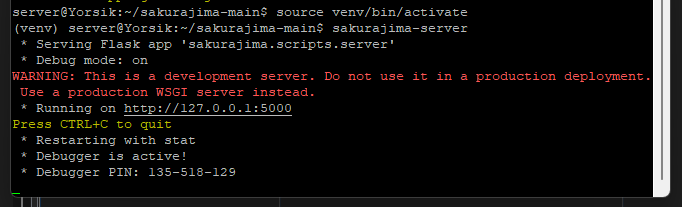
\includegraphics[width=.9\textwidth]{graphics/test/dev_server_run.png}
  \caption{Демонстрация информации о статусе запуска сервера (Flask)}
  \label{fig:test0}
\end{figure}

Проведем тестирование заявленного функционала.

\section{Создание модуля}

Для создания модуля следует создать папку с названием соответствующего модуля в нужном месте. Внутри этой папки следует разместить файл module.json, в котором указываются имя и версия модуля. Возьмем для примера модуль с названием demo версии 1.0.0. Внешний вид папки модуля представлен на рисунке~\ref{fig:test1}.

\begin{figure}
  \centering
  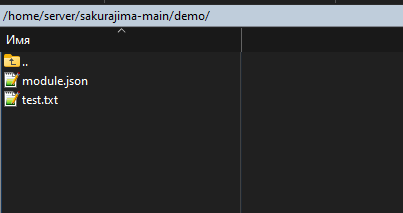
\includegraphics[width=.6\textwidth]{graphics/test/demo_r.png}
  \caption{Содержимое папки модуля demo}
  \label{fig:test1}
\end{figure}
\newpage
\section{Отправка модуля}

Впоследствии, выполняем команду sakurajima upload demo, которая загружает модуль под названием demo на сервер, выполнение команды представлено на рисунке~\ref{fig:test2}. 

\begin{figure}
  \centering
  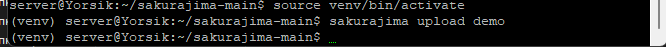
\includegraphics[width=1.0\textwidth]{graphics/test/demo.png}
  \caption{Выполнение команды отправки модуля на сервер в CLI}
  \label{fig:test2}
\end{figure}

В итоге, на сервере появляется конкретная версия модуля и последняя версия, рисунке~\ref{fig:test3}. 

\begin{figure}
  \centering
  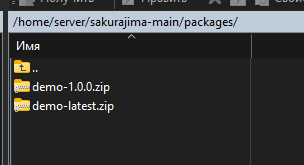
\includegraphics[width=.7\textwidth]{graphics/test/demo_alias_modules.png}
  \caption{Содержимое папки модулей на сервере}
  \label{fig:test3}
\end{figure}

\section{Обновление модуля}

Модифицируем версию модуля в файле и добавляем дополнительный файл - изображение. Затем повторно активизируем команду sakurajima upload demo, результат команды представлен на рисунке~\ref{fig:test4}. 

\begin{figure}
  \centering
  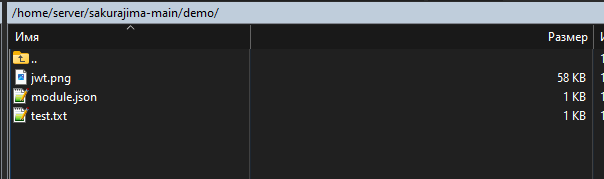
\includegraphics[width=.8\textwidth]{graphics/test/demo_jwt.png}
  \caption{Обновленное содержимое папки модуля demo}
  \label{fig:test4}
\end{figure}

\newpage

Теперь у нас имеется две версии - 1.0.0 и 1.5.0. Результат выполнения команды представлен на рисунке \ref{fig:test5}.

\begin{figure}
  \centering
  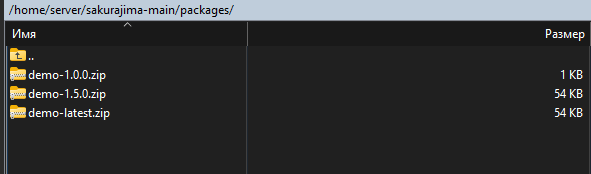
\includegraphics[width=.8\textwidth]{graphics/test/demo_jwt_final.png}
  \caption{Обновленное содержимое папки модулей на сервере}
  \label{fig:test5}
\end{figure}

\section{Загрузка модуля}

Для проверки функционирования загрузки модуля demo, предварительно удалим локально.

Используем следующую команду: sakurajima install name-module==version

Стандартная процедура установки предусматривает установку самой последней версии модуля (latest). Результат выполнения команды представлен на рисунке \ref{fig:test6}.

\begin{figure}
  \centering
  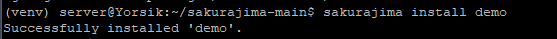
\includegraphics[width=.8\textwidth]{graphics/test/dev_install.png}
  \caption{Результат выполнения команды установки модуля demo}
  \label{fig:test6}
\end{figure}

Если мы укажем через `==` версия, то будет загружена определенная версия модуля. Результат выполнения команды представлен на рисунке \ref{fig:test7}.

\begin{figure}
  \centering
  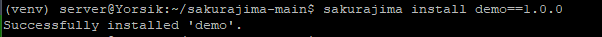
\includegraphics[width=.8\textwidth]{graphics/test/dev_install_ver.png}
  \caption{Результат выполнения команды установки модуля demo с конкретной версией}
  \label{fig:test7}
\end{figure}

\newpage

\section{Удаление модуля}

Используем команду: sakurajima uninstall name-module, результат команды представлен на рисунке~\ref{fig:test8}. 

\begin{figure}
  \centering
  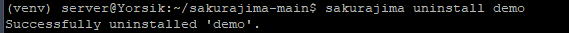
\includegraphics[width=.8\textwidth]{graphics/test/dev_uninstall.png}
  \caption{Результат выполнения команды удаления модуля demo}
  \label{fig:test8}
\end{figure}

\section{Проверка модуля на увязвимости}

Используем команду: sakurajima cve

Команда cve предназначена для выполнения поиска уязвимостей. Эта команда анализирует все установленные пакеты, выявляет потенциально уязвимые версии и предоставляет подробные рекомендации по устранению обнаруженных уязвимостей.

\section{Система зависимостей в модулях}

Реализация зависимостей представлена на рисунке \ref{fig:test9}.

\begin{figure}
  \centering
  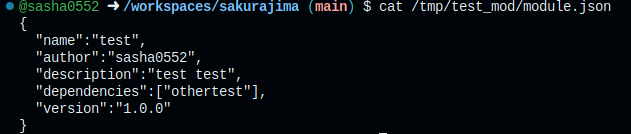
\includegraphics[width=.8\textwidth]{graphics/test/info2.png}
  \caption{Содержимое тестового модуля с указанием зависимостей (dependencies)}
  \label{fig:test9}
\end{figure}

\section{Информирование о модуле}

Используем команду: sakurajima info

Информация о модуле представлена на рисунке \ref{fig:test10}.

\begin{figure}
  \centering
  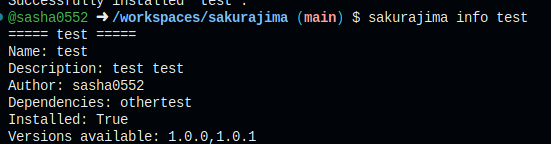
\includegraphics[width=.8\textwidth]{graphics/test/info3.png}
  \caption{Результат команды для установленного локально модуля}
  \label{fig:test10}
\end{figure}


%%% Local Variables:
%%% mode: latex
%%% TeX-master: "rpz"
%%% End:
